\chapter{Skalarprodukt}
\section{Definitionen}
\subsection{Skalarprodukt}
\label{sec:6.1}
Seien $\vec{u} = \varvektor{c}{u_1\\u_2\\\vdots\\u_n}$, $\vec{v} = \vektor{\vec{v_1}}{\vdots}{v_n} \in \mathbb{R}^n$, dann ist das Skalarprodukt\index{Skalarprodukt} der Vektoren $\vec{u}$ und $\vec{v}$ definiert durch
\begin{align*}
	\vec{u} \mal \vec{v} :&= (\vec{u})^T \vec{v} = \left(u_1, \dots, u_n\right) \mal \vektor{v_1}{\vdots}{v_n}\\
	&= u_1 \mal v_1 + u_2 \mal v_2 + \dots + u_n v_n = \sumx{k = 1}{n}{u_k \mal v_k \in \mathbb{R}}
\end{align*}
\bsp{Bemerkung:}{
\begin{enumerate}
\item Skalarprodukt\index{Skalar}, da das Resultat ein Skalar ist
\item \begin{itemize}[leftmargin=\widthof{2. }]
		\item z.T wird das Skalarprodukt auch inneres Produkt genannt.
		\item englische Bezeichnung ''dot product'' (Maple DotProduct)
		\end{itemize}
\item Das Skalarprodukt ist ein Spezialfall der Matrizenmultiplikation.
\end{enumerate}}

\subsection{Norm}
\label{sec:6.3}
Sei $\vec{u} \in \mathbb{R}^n$, dann ist die (euklidische) Norm\index{Norm} von $\vec{u}$ gegeben durch
\[\| \vec{u} \| = \sqrt{\vec{u} \mal \vec{u}} = \sqrt{u_1^2 + u_2^2 + \dots + u_n^2}\]
\bsp{Bemerkung:}{
\begin{enumerate}
\item statt $\| \vec{u} \|$ schreibt man manchmal $\left| \vec{u} \right|$
\item $\| \vec{u} \|$ entspricht der geometrischen L�nge des Vektors $\vec{u}$\\
%14.01.2009-IMG-mathe-1
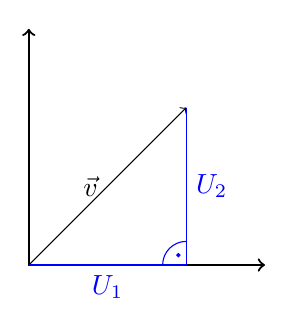
\begin{tikzpicture}
	\draw[thick, <->] (3,0) -- (0,0) -- (0,3);

	\draw[->] (0,0) -- (2,2) node[left, midway] {$\vec{v}$};
	\draw[draw=blue, thick] (0,0) -- (2,0) node[below, midway, text=blue] {$U_1$};
	\draw[draw=blue] (2,0) -- (2,2) node[right, midway, text=blue] {$U_2$};
	\draw[draw=blue] (1.7,0) arc (180:90:0.3);
	\draw[draw=blue, fill=blue] (1.9,0.125) circle (0.02);
\end{tikzpicture}\\
Pythagoras $\| \vec{u} \| = \sqrt{u_1^2 + u_2^2}$
\item Der Abstand zwischen zwei Punkten $A$ und $B$ (mit Ortsvektoren $\vec{a}$ bzw. $\vec{b}$ ist gleich der L�nge des Vektors $\vec{AB} = \vec{b} - \vec{a}$
		\[d\left(\vec{a}, \vec{b}\right) = \| \vec{b} - \vec{a} \| = \| \vec{a} - \vec{b} \|\]
\end{enumerate}}

\subsection{Orthogonalit�t}
\label{sec:6.6}
Zwei Vektoren $\vec{u}, \vec{v} \in \mathbb{R}^n$ nennt man orthogonal\index{orthogonal} bzw. senkrecht bzw. rechtwinklig wenn
\[\vec{u} \mal \vec{v} = 0\]
%15.01.2009-IMG-mathe-1
\begin{tikzpicture}
	\draw[<->, thick] (0,3) -- (0,0) node[left, midway] {$\vec{v}$} -- (5,0) node[below, midway] {$\vec{u}$};
	\draw[thick] (0,0.5) arc (90:0:0.5);
	\path (0,0) ++(45:0.25) node{$\alpha$};
\end{tikzpicture}

$\alpha = 90� \Ra \cosx{\alpha} = 0$

Man schreibt dann auch $\vec{u} \perp \vec{v}$.

\section{S�tze}
\subsection{Eigenschaften des Skalarproduktes}
\label{sec:6.2}
Seien $\vec{u}, \vec{v}, \vec{w} \in \mathbb{R}^n$, $\lambda \in \mathbb{R}$, dann gilt:
\begin{enumerate}[label=\roman*)]
\item Kommutativgesetz: $\vec{u} \mal \vec{v} = \vec{v} \mal \vec{u}$
\item Distributivgesetz: $\vec{u} \mal \left(\vec{v} + \vec{w}\right) = \vec{u} \mal \vec{v} + \vec{u} \mal \vec{w}$
\item $\left(\lambda \mal \vec{u}\right) \vec{v} = \lambda \mal \left(\vec{u} \mal \vec{v}\right) = \vec{u} \mal \left(\lambda \vec{v}\right)$
\item $\vec{u} \mal \vec{u} \geq 0$\\
		$\vec{u} \mal \vec{u} = 0 \Lra \vec{u} = \vec{0}$
\end{enumerate}
\bsp[nachrechnen]{Beweis:}

\subsection{Eigenschaften der Norm}
\label{sec:6.4}
Seien $\vec{u}, \vec{v} \in \mathbb{R}^n$, $\lambda \in \mathbb{R}$, dann gilt
\begin{enumerate}[label=\roman*)]
\item $\| \vec{u} \|^2 = \vec{u} \mal \vec{u}$
\item Homogenit�t: $\| \lambda \vec{u} \| = \left| \lambda \right| \mal \| \vec{u} \|$
\item $\| \vec{u} \| = 0 \Lra \vec{u} = 0$
\item Normierbarkeit: jedem Vektor $\vec{u} \neq \vec{0}$ kann ein normierter\index{Normierter} Vektor $\vec{v}$ zugewiesen werden mit $\vec{v} = \frac{1}{\| \vec{u} \|} \mal \vec{u}$ und $\| \vec{v} \| = 1$
\end{enumerate}
\bsp[nachrechnen]{Beweis:}

\subsection{Satz}
\label{sec:6.5}
Das Skalarprodukt zweier Vektoren $\vec{u}, \vec{v} \in \mathbb{R}^n$ kann man auch berechnen durch
\[\vec{u} \mal \vec{v} = \| \vec{u} \| \mal \| \vec{v} \| \mal \cosx{\alpha}\]
mit $\alpha$ als Winkel zwischen $\vec{u}$ und $\vec{v}$

%14.01.2009-IMG-mathe-2
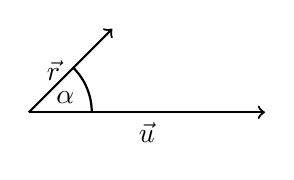
\begin{tikzpicture}
	\draw[->, thick] (0,0) -- (3,0) node[below, midway] {$\vec{u}$};
	\draw[->, thick] (0,0) -- (45:1.5) node[left, midway] {$\vec{r}$};
	\draw[thick] (0.8,0) arc (0:45:0.8);
	\path (0,0) ++(22.5:0.5) node{$\alpha$};
\end{tikzpicture}
%14.01.2009-IMG-mathe-3
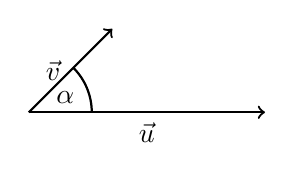
\begin{tikzpicture}
	\draw[->, thick] (0,0) -- (3,0) node[below, midway] {$\vec{u}$};
	\draw[->, thick] (0,0) -- (45:1.5) node[left, midway] {$\vec{v}$};
	\draw[thick] (0.8,0) arc (0:45:0.8);
	\path (0,0) ++(22.5:0.5) node{$\alpha$};
\end{tikzpicture}
%14.01.2009-IMG-mathe-4
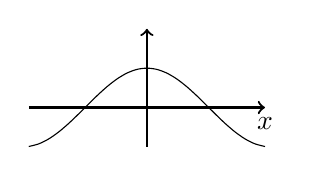
\begin{tikzpicture}
	\draw[->, thick] (-1.5,0) -- (1.5,0) node[below] {$x$};
	\draw[->, thick] (0,-0.5) -- (0,1);
	\draw[smooth] plot[domain=-3:3, scale=0.5] (\x,{cos(\x r)});
\end{tikzpicture}

\bsp[Winkel zwischen $\vec{u}$ und $\vec{v}$]{Beispiel:}{
Test Test Test
$\vec{u} \mal \vec{v} = \sumx{k = 1}{n}{u_k \mal v_k} = \| \vec{u} \| \mal \| \vec{v} \| \mal \cosx{\alpha}$\\
$\Lra \cosx{\alpha} = \frac{\vec{u} \mal \vec{v}}{\| \vec{u} \| \mal \| \vec{v} \|}$\\
$\Ra \alpha = \arccosx{\frac{\vec{u} \mal \vec{v}}{\| \vec{u} \| \mal \| \vec{v} \|}}$}

\subsection{Pythagoras}
\label{sec:6.7}
Seien $\vec{u}, \vec{v} \in \mathbb{R}^n$ dann gilt:
\[\vec{u} \perp \vec{v} \Lra \| \vec{u} + \vec{v} \| = \| \vec{u} \|^2 + \| \vec{v} \|^2\]
%15.01.2009-IMG-mathe-2
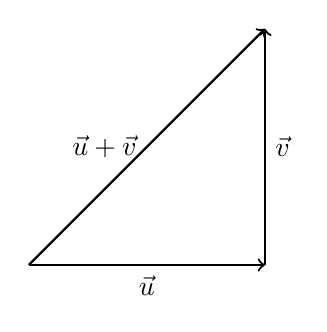
\begin{tikzpicture}
	\draw[->, thick] (0,0) -- (3,3) node[left, midway] {$\vec{u} + \vec{v}$};
	\draw[->, thick] (0,0) -- (3,0) node[below, midway] {$\vec{u}$};
	\draw[->, thick] (3,0) -- (3,3) node[right, midway] {$\vec{v}$};
\end{tikzpicture}

\bsp{Beweis:}{
\begin{align*}
	\| \vec{u} + \vec{v} \|^2 &= \left(\vec{u} + \vec{v}\right) \mal \left(\vec{u} + \vec{v}\right)\\
	&= \vec{u} \mal \left(\vec{u} + \vec{v}\right) + \vec{v} \mal \left(\vec{u} + \vec{v}\right)\\
	&= \vec{u} \mal \vec{u} + \vec{u} \mal \vec{v} + \vec{v} \mal \vec{u} + \vec{v} \mal \vec{v}\\
	&= \| \vec{u} \|^2 + \| \vec{v} \|^2 + 2 \underbrace{(\vec{u} \mal \vec{v})}_{= 0 \Lra \vec{u} \perp \vec{v}}\\
	&= \| \vec{u} \|^2 + \| \vec{v} \|^2
\end{align*}
%15.01.2009-IMG-mathe-3
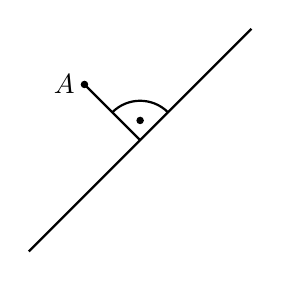
\begin{tikzpicture}
	\draw[thick] (0,0) -- (45:4);
	\draw[thick] (45:2) -- +(135:1);
	\draw[fill=black] (45:2) ++ (135:1) circle (0.04) node[left] {$A$};
	\draw[thick] (45:2) ++ (135:0.5) arc (135:45:0.5);
	\draw[fill=black] (45:2) ++ (90:0.25) circle (0.04);
\end{tikzpicture}
}

\section{Aufgaben}
\subsection{Aufgabe 5.1}
\label{sec:Aufgabe-EukVektorraum-A5.1}
Bestimmen sie die Menge $F$ aller Vektoren $\vec{v} \in \mathbb{R}^3$, f�r die gilt $\vec{v} \perp \vec{u} = \vektor{-1}{2}{3}$

L�sung siehe \vref{sec:Loesung-EukVektorraum-A5.1}.

\subsection{Aufgabe 5.2}
\label{sec:Aufgabe-EukVektorraum-A5.2}
Zeigen sie unter Verwendung des Skalarproduktes, dass das folgende Dreieck rechtwinklig ist:
\[A := \vektor{3}{-2}{12}, B := \vektor{7}{0}{11}, C := \vektor{6}{-7}{14}\]
L�sung siehe \vref{sec:Loesung-EukVektorraum-A5.2}.
